\documentclass[conference,a4paper]{IEEEtran}
\IEEEoverridecommandlockouts
\usepackage[left=1.57cm,right=1.57cm,top=0.95cm,bottom=2.54cm]{geometry}
\newpage % Mulai halaman kedua
% \usepackage{caption}

% \captionsetup[figure]{justification=raggedright, singlelinecheck=off}

% Mengubah margin pada halaman kedua
\newgeometry{left=1.57cm,right=1.57cm,top=1.9cm,bottom=2.54cm}
% The preceding line is only needed to identify funding in the first footnote. If that is unneeded, please comment it out.
\usepackage{cite}
\usepackage{amsmath,amssymb,amsfonts}
\usepackage{algorithmic}
\usepackage{graphicx}
\usepackage{textcomp}
\usepackage{xcolor}
\usepackage{balance}
\usepackage{multirow}
\usepackage{enumitem}
\def\BibTeX{{\rm B\kern-.05em{\sc i\kern-.025em b}\kern-.08em
    T\kern-.1667em\lower.7ex\hbox{E}\kern-.125emX}}
\begin{document}

\title{
  Development of RWikiStat 4.0: A Multiplatform Application for Learning Basic Statistics Using the Rapid Application Development Method \\
}

\makeatletter
\newcommand{\linebreakand}{
  \end{@IEEEauthorhalign}
  \hfill\mbox{}\par
  \mbox{}\hfill\begin{@IEEEauthorhalign}
}
\makeatother

\author{
  Hizir Sofyan\textsuperscript{1}, Munawar\textsuperscript{1}, Muhammad Subianto\textsuperscript{2}, Kurnia Saputra\textsuperscript{2*},\\
  Naufal Mas Adha\textsuperscript{2}, Affan Ian Amara\textsuperscript{2}, Muhammad Nurifai\textsuperscript{2}, Akhyar\textsuperscript{2}\\
  \\
  \textsuperscript{1}Department of Statistics, Universitas Syiah Kuala, Banda Aceh, Indonesia\\
  \textsuperscript{2}Department of Informatics, Universitas Syiah Kuala, Banda Aceh, Indonesia\\
  *Corresponding Author: kurnia.saputra@usk.ac.id
}

\maketitle

\begin{abstract}
  RWikiStat is a multiplatform application developed to support the learning process of basic statistics in a more interactive and applicable way. This application is designed to help students understand statistical concepts through structured materials, practice questions, and data visualization. RWikiStat was developed using the Rapid Application Development (RAD) method which consists of four stages: Planning, User Design, Construction, and Cutover.

  The test results show that RWikiStat successfully meets the functional needs of users and provides a good user experience, with a user satisfaction level of 88.26\%. Testing was carried out through functional testing and usability testing to ensure that all features function properly and the system interface is easy to use. RWikiStat supports an active learning process, where users not only read the material, but also directly test their understanding through the available exercises. This application has great potential as an effective learning medium in higher education environments.

\end{abstract}

\begin{IEEEkeywords}
  RWikiStat 4.0, Multiplatform application, Basic statistics, Interactive learning.
\end{IEEEkeywords}

\section{Introduction}
\label{sect:introduction}

In the practice of learning statistics, there are still several challenges faced by students. Starting from challenges that arise from themselves, lecturers, the environment, and facilities and infrastructure. According to Deci and Dewi \cite{b1}, the facilities and infrastructure factor is the most influential factor in the teaching and learning process. This is also in accordance with the statement of Wild and Pfannkuch \cite{b2} who define that the lack of learning materials that can help students to practice and apply statistical thinking is a major problem in the practice of learning statistics. Traditional passive learning is considered less than optimal in describing the relationship between statistics and real-world applications. On the other hand, learning with the use of technology can help increase students enthusiasm for learning, such as in Serina's research which explored the challenges in teaching statistics by using Microsoft Excel as a teaching and learning tool. The statistical learning process carried out received a positive response and a high level of enthusiasm from students. This describes the opportunities to integrate various other technologies in helping statistical learning \cite{b3}.

Various technologies can be utilized to assist in the learning process, such as the use of the web and mobile devices. Although various applications have been developed, many still have limitations in terms of interactivity, accessibility, and feature integration. Therefore, a solution was developed that can answer the problems in learning statistics by utilizing technology in the learning process. RWikiStat is present as a solution that combines learning modules, R compilers, chatbots, discussion forums, and customizable settings, offering a new approach to learning statistics that is more effective and efficient. RWikiStat is a statistics learning application that is now available in website versions and mobile applications based on Android and iOS.

RWikiStat was first launched as an interactive platform for learning statistics in 2010 by integrating a wiki application \cite{b4}. Development continued with the launch of RWikiStat 2.0 which is open-source and developed in the Linux environment \cite{b5}. Then in 2019 the third version was developed in the form of an Android application \cite{b6}. This development was perfected in 2024 to optimize all existing features. This version was developed using a combination of React Native and Expo so that it can run on Android and iOS platforms.

\section{Methodology}
\label{sect:methodology}

Rapid Application Development (RAD) method was used in this research. This method was chosen because it has the ability to reuse existing components so that the time range can be shorter \cite{b7}. Furthermore, it reduces costs through focused development and has satisfactory results according to stakeholder feedback provided during the development process \cite{b8}. RAD has 4 stages which are requirements planning, user design, rapid construction, and implementation as can be seen in Figure~\ref{method}.

\begin{figure}[htb]
  \centering
  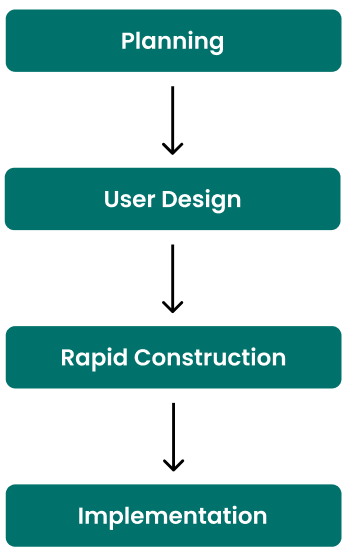
\includegraphics [width=3 cm, height=4.5 cm]{images/method}
  \caption{Research Methodology Flow Diagram}
  \label{method}
\end{figure}

\begin{enumerate}
  \item Planning
  \item[] In this stage, problem identification is carried out by discussing with stakeholders to determine the needs that are the basis for designing the system. These needs are the basis for designing and developing features in the application. From this process, a requirement specification is produced which includes the main features that must be present in the application. In addition, the target users for the system being developed are obtained, who are students of basic statistics courses.

        In addition, at this stage, the tools to be used were also agreed upon. To develop a multiplatform application, several frameworks were used, starting from Next.js for the website version, a combination of Expo and React Native for the mobile version, and Express.js as the application backend. Next.js was chosen because it has static site generation and optimized builds result in faster page loads \cite{b9}. Because of the need for fast development with the same results on Android and iOS platforms, Expo React Native is the best answer by providing a native look and fast reload \cite{b10}. Then, to store all data so that it is well organized, Express.js was chosen to build the application backend because it allows fast and efficient development \cite{b11}.

  \item User Design
  \item [] At the user design stage, an application prototype design is carried out based on the previous stage. The application design in the form of a user interface (UI) and prototype is created using the Figma tool. The prototype of this application will then be tested to evaluate its suitability to user desires. Then, all prototypes that have been tested will be adjusted again based on suggestions given by the user. The final result of this stage is an application design that includes all pages, navigation, and logical flows that will be implemented for the next stage.

  \item Rapid Construction
  \item [] In the rapid construction stage, the previously designed system is built. The system is built using agreed languages and frameworks, starting from database development, frontend, and backend. Through this stage, the finalized design is transformed into a usable application. In this stage, feedback collection from users is also continuously carried out to ensure that the system built is in accordance with desires.

  \item Implementation
  \item [] At the implementation stage, a thorough test is carried out on the system to ensure that there are no errors when implementing the system that has been built. Researchers use two testing methods, namely testing the system's functionality using black box testing to reduce the possibility of system defects and testing the system's usability using the Usability Metric for User Experience (UMUX) to measure the level of user satisfaction in using the system that has been built.


\end{enumerate}

\section{Results and Discussion}
\label{sect:results_discussion}

The statistics learning application, RWikiStat has been developed on all platforms starting from the website, Android and iOS with features that can help learning. RWikiStat provides a statistics learning module equipped with sample questions and code samples so that users can directly practice the statistical concepts that have been learned. In addition to trying the code samples available in each module, users can also access the compiler and try various statistical codes in the R language to strengthen their understanding. The compiler that has been equipped with Shiny integration allows users to try to visualize the desired statistical data. Furthermore, RWikiStat provides a discussion forum that can be used to ask or answer questions that are understood. Then there is also a chatbot feature so that users can ask about statistical problems without having to move to another platform.

To ensure that the system runs according to user desires, two testing processes are carried out, namely functionality testing and usability testing.

\begin{enumerate}[label=\alph*.]
  \item Functionality Testing
  \item [] Functional testing is done using black box testing to test the application in various desired scenarios. This testing is done to see the functions contained in the system. From all the features tested, all features were found to run well according to the expected scenario.

  \item Usability Testing
  \item [] Usability testing conducted using the UMUX method aims to test whether the system can be understood and used by users. Before conducting the test, a test plan application is prepared which can be seen in Table~\ref{tab:test_plan}.

        \begin{table}[htbp]
          \caption{Test Plan Application}
          \label{tab:test_plan}
          \resizebox{\columnwidth}{!}{%
            \begin{tabular}{|l|}
              \hline
              \multicolumn{1}{|c|}{{\color[HTML]{333333} \textbf{Test Plan Application}}} \\ \hline
              {\color[HTML]{333333}
                \begin{tabular}[c]{@{}l@{}}
                  Scenario:                                                      \\
                  - The user opens the application.                              \\
                  - The user understands the appearance of the home page.        \\
                  - The user logs into the application.                          \\
                  - The user accesses the learning modules.                      \\
                  - The user reads the available learning modules.               \\
                  - The user downloads the available learning modules.           \\
                  - The user tries to compile R code.                            \\
                  - The user tries to ask the chatbot a question.                \\
                  - The user tries to post a question in the discussion forum.   \\
                  - The user tries to answer a question in the discussion forum. \\
                  - The user tries to save a post.                               \\
                  - The user tries to like a post.                               \\
                  - The user tries to view their post history.                   \\
                  - The user tries to delete their own question.                 \\
                  - The user tries to sign out of the application.
                \end{tabular}
              }                                                                           \\ \hline
              {\color[HTML]{333333}
                \begin{tabular}[c]{@{}l@{}}Tool:\\ - iOS Smartphone\end{tabular}
              }                                                                           \\ \hline
            \end{tabular}%
          }
        \end{table}

        Respondents will run the application according to the test plan that has been made. Respondents for this test consisted of 22 students of basic statistics courses. After that, respondents were asked to fill out a questionnaire form with questions as shown in Table~\ref{tab:umux_question_list}.

        \begin{table}[htbp]
          \caption{UMUX QUESTION LIST \cite{b12}}
          \label{tab:umux_question_list}
          \resizebox{\columnwidth}{!}{%
            \begin{tabular}{|c|l|c|}
              \hline
              \textbf{No.} & \textbf{Question}                                      & \textbf{Score} \\ \hline
              1            & This application suits my needs.                       & 1 - 7          \\ \hline
              2            & I had a bad experience using this application.         & 1 - 7          \\ \hline
              3            & This application is easy to use.                       & 1 - 7          \\ \hline
              4            & I have to spend a lot of time to use this application. & 1 - 7          \\ \hline
            \end{tabular}%
          }
        \end{table}
\end{enumerate}



After testing using the UMUX method, the test result data is processed following these steps:
\begin{itemize}
  \item Each odd-numbered item is calculated using the formula [user score- 1], while even-numbered items are calculated using the formula [7- user score].
  \item The scores of each item filled in by the user are added up first, then divided by 24 (the maximum score value).
  \item The result of the division is multiplied by 100.
  \item Furthermore, the value is averaged for all users.
  \item The UMUX score obtained is assessed on a scale of 0-100, according to general assessment standards\cite{b13}.
\end{itemize}

The results of the tests carried out using the UMUX method can be seen in Table~\ref{tab:umux_results}.

\begin{table}[htbp]
  \caption{UMUX Testing and Evaluation Results for the RWikiStat Application}
  \label{tab:umux_results}
  \resizebox{\columnwidth}{!}{%
    \begin{tabular}{|l|c|c|c|c|c|}
      \hline
      \multirow{2}{*}{\textbf{Respondent}}   & \multicolumn{4}{c|}{\textbf{Question Number}} & \multirow{2}{*}{\textbf{Final Score}}                                   \\ \cline{2-5}
                                             & \textbf{1}                                    & \textbf{2}                            & \textbf{3} & \textbf{4} & ~     \\ \hline
      Chemistry Student 2                    & 4                                             & 1                                     & 7          & 1          & 87,5  \\ \hline
      Chemistry Student 3                    & 4                                             & 1                                     & 6          & 2          & 79,17 \\ \hline
      Chemistry Student 4                    & 7                                             & 1                                     & 7          & 3          & 91,67 \\ \hline
      Chemistry Student 5                    & 6                                             & 2                                     & 5          & 3          & 75    \\ \hline
      Chemistry Student 6                    & 7                                             & 1                                     & 7          & 1          & 100   \\ \hline
      Informatics Student 1                  & 7                                             & 2                                     & 7          & 1          & 95,83 \\ \hline
      Informatics Student 2                  & 7                                             & 1                                     & 7          & 1          & 100   \\ \hline
      Informatics Student 3                  & 7                                             & 1                                     & 7          & 1          & 100   \\ \hline
      Informatics Student 4                  & 7                                             & 2                                     & 6          & 2          & 87,5  \\ \hline
      Informatics Student 5                  & 7                                             & 1                                     & 7          & 2          & 95,83 \\ \hline
      Informatics Student 6                  & 7                                             & 2                                     & 5          & 2          & 83,33 \\ \hline
      Informatics Student 7                  & 7                                             & 1                                     & 7          & 1          & 100   \\ \hline
      Biology Student 1                      & 5                                             & 1                                     & 7          & 5          & 75    \\ \hline
      Biology Student 2                      & 7                                             & 1                                     & 7          & 4          & 87,5  \\ \hline
      Biology Student 3                      & 7                                             & 1                                     & 7          & 1          & 100   \\ \hline
      Biology Student 4                      & 6                                             & 1                                     & 7          & 1          & 95,83 \\ \hline
      Biology Student 5                      & 5                                             & 1                                     & 7          & 1          & 91,67 \\ \hline
      Biology Student 6                      & 4                                             & 1                                     & 4          & 2          & 70,83 \\ \hline
      Biology Student 7                      & 6                                             & 2                                     & 6          & 6          & 66,67 \\ \hline
      Biology Student 8                      & 7                                             & 1                                     & 7          & 5          & 83,33 \\ \hline
      Biology Student 9                      & 6                                             & 1                                     & 6          & 4          & 75    \\ \hline

      \multicolumn{5}{|c|}{\textbf{Average}} & \textbf{88.26}                                                                                                          \\ \hline
    \end{tabular}%
  }
\end{table}

Based on the test results in Table~\ref{tab:umux_results}, an average value of 88.26\% was obtained. This shows that the RWikiStat application has an interpretation score of "Best Imaginable" with a grade of "A" using the UMUX calculation method.



\section{Conclusions and Suggestions}
\label{sect:conclusion}

In this paper, we introduce an interactive statistics learning application, RWikiStat, to increase student interest in learning statistics. This application has features that can facilitate students in learning, such as the existence of learning modules equipped with sample questions along with sample codes for each material, allowing students to try it directly. There is also a discussion forum that can create interactive and interesting learning. Moreover, chatbot features and compiler features equipped with Shiny implementation to visualize data statistically are also available in this application. This allows users to understand statistical concepts in an interesting way. RWikiStat is also available for all platforms, which are websites, Android and iOS, thus expanding the scope of users who can use it. To ensure that all features run according to the plan, we have conducted functionality testing using the black box testing method. In this test, it was found that all features can run properly. In addition, usability testing was also carried out to ensure that this application can be used easily by users. The results of this test found that the level of satisfaction of respondents who were students of introductory statistics courses was 88.26\%, which indicates “Best Imaginable” with grade “A” using the UMUX calculation method.

In conclusion, RWikiStat application has proven to be user-friendly and has the potential to become a tool in the field of statistics. Further development for this application can be done by providing multi-language features and allowing offline access by users.


\balance

\begin{thebibliography}{00}

  \bibitem{b1}Ririen, Deci, and Dewi Hartika. "Identifikasi Kesulitan Belajar Mahasiswa pada Mata Kuliah Statistika Selama Masa Pandemi Covid-I9." Jurnal Ilmiah Universitas Batanghari Jambi 21.1 (2021): 148-155.

  \bibitem{b2}Wild, Chris J., and Maxine Pfannkuch. "Statistical thinking in empirical enquiry." International statistical review 67.3 (1999): 223-248.

  \bibitem{b3}Uchima-Marin, Cristian, et al. "Integration of Technological Tools in Teaching Statistics: Innovations in Educational Technology for Sustainable Education." Sustainability 16.19 (2024): 8344.

  \bibitem{b4}Subianto, Muhammad, and Hizir Sofyan. "Interactive statistics learning with RWikiStat." 2010 International Conference on Networking and Information Technology. IEEE, 2010.

  \bibitem{b5}Sofyan, Hizir, Edi Muttaqin, and Muhammad Subianto. "RWikiStat 2.0: a Web Based Statistical Learning System (Session 1B (IASC-ARS))." Proceedings of the symposium of Japanese Society of Computational Statistics 26. Japanese Society of Computational Statistics, 2012.

  \bibitem{b6}Sofyan, Hizir, et al. "Analisis Kepuasan Pengguna Aplikasi RWikiStat 3.0." Journal of Data Analysis 2.2 (2020): 80-87.

  \bibitem{b7}Anggraini, Lili. "The Impact of New Media in the Information Society Era." Journal of Information Systems and Management (JISMA) 2.2 (2023): 29-33.

  \bibitem{b8}Paulsen, June Blydt, and Helle Låhne Smedsrud. The" Good Enough" Tsunami: The Disruptive Potential of Low-code and No-code: A multiple case-study on scope, trends, and implications. MS thesis. 2023.

  \bibitem{b9}Svedas, Egidijus. "Building an application using Next. js." (2024).

  \bibitem{b10}Nitschke, Marlies, et al. "Refinement and usability analysis of an eHealth app for ankylosing spondylitis as a complementary treatment to physical therapy: development and usability study." JMIR Formative Research 7 (2023): e47426.

  \bibitem{b11}Azkarin, Varinia, Rangga Gelar Guntara, and Oding Herdiana. "Development of a REST API for Human Resource Information System for Employee Referral Management Domain Using the Express JS Framework and Node. js." Journal of Scientific Research, Education, and Technology (JSRET) 2.3 (2023): 1085-1094.

  \bibitem{b12}Lewis, James R., and Jeff Sauro. "Usability and user experience: Design and evaluation." Handbook of human factors and ergonomics (2021): 972-1015.

  \bibitem{b13}Finstad, Kraig. "The usability metric for user experience." Interacting with computers 22.5 (2010): 323-327.

\end{thebibliography}

\end{document}